\documentclass[11pt,a4paper]{ltjsarticle}

\usepackage{amsmath,amssymb}
\usepackage{graphicx}
\usepackage{hyperref}
\usepackage{geometry}
\usepackage{tikz}
\usetikzlibrary{arrows.meta,calc,positioning,shapes.geometric}

\geometry{margin=25mm}
\hypersetup{
  colorlinks=true,
  linkcolor=blue,
  urlcolor=blue
}
\tikzset{
  block/.style={
    draw,
    rounded corners=2pt,
    align=center,
    minimum width=30mm,
    minimum height=10mm,
    fill=gray!8
  },
  line/.style={
    -{Latex[length=2.2mm,width=1.4mm]},
    thick
  },
  decision/.style={
    draw,
    diamond,
    aspect=2,
    align=center,
    inner sep=1pt,
    minimum width=22mm,
    fill=gray!8
  },
  terminator/.style={
    draw,
    rounded corners=6pt,
    align=center,
    minimum width=22mm,
    minimum height=8mm,
    fill=gray!8
  }
}

\title{提案手法メモ１}
\author{}
\date{\today}

\setcounter{tocdepth}{2}

\begin{document}

\maketitle
\tableofcontents
\clearpage

% Generated from notes/paper_sections_3_4_full_draft.md

\section{3. 提案手法}


\subsection{3.1 提案法の基本的な考え方}


遺伝的プログラミングにおける交叉率 $p_c$ と突然変異率 $p_m$ は、探索の多様性、収束速度、最終性能に強く影響する重要な操作パラメータである。しかし、従来の GP ではこれらの値を全世代を通じて固定する場合が多く、探索初期と収束期で異なる操作特性が望まれる可能性を十分に取り込めない。とくに、多目的 GP では、単に最終性能のみを高めるだけでなく、進化の途中で多様性を保ちつつ探索を進める必要があるため、固定率の限界はより顕著になる。

本研究では、この問題を静的なハイパーパラメータ調整の問題としてではなく、進化状態を観測しながら操作入力を逐次更新する制御問題として捉える。すなわち、GP 本体を状態遷移を生むプラント、外側のベイズ最適化を制御器とみなし、現在の探索状態に応じて次区間で用いる操作率を決定する閉ループ構造を導入する。

提案法の本質は、交叉率 $p_c$ と突然変異率 $p_m$ を可変にすること自体ではない。提案法では、これら 2 つの操作率に加えて、次回更新までの世代数 $k$ も制御対象に含める。これにより、提案法は「どの程度の操作強度を与えるか」だけでなく、「いつ再調整するか」も状態依存で切り替える文脈付き制御として定式化される。

\subsection{3.2 閉ループ制御としての定式化}


世代 $g$ における GP 集団を $P_g$ とする。また、外側 BO による制御更新の回数を $\ell$ で表す。提案法では、制御ステップ $\ell$ において

\[
u_\ell = (p_{c,\ell}, p_{m,\ell}, k_\ell)
\]

を決定し、その値を $k_\ell$ 世代のあいだ保持して GP を進化させる。したがって、連続する更新時点の世代番号は

\[
g_{\ell+1} = g_\ell + k_\ell
\]

で与えられる。ここで、$g$ は GP の世代時間、$\ell$ は BO が介入する外側制御時間を表しており、提案法は二重時間軸を持つ。

GP の進化作用全体を $F$、進化計算に固有の確率的ゆらぎを $\xi_\ell$ とすると、制御区間 $\ell$ における集団遷移は

\[
P_{g_{\ell+1}} = F(P_{g_\ell}, u_\ell, \xi_\ell)
\]

と表せる。この式において、GP は入力 $u_\ell$ を受けて状態を変化させるプラントであり、BO は現在の状態を観測して次の入力を決める制御器として機能する。ここでの観測とは、単一の性能値だけを見ることではなく、進化段階、改善速度、多様性、複雑度、停滞状況を含む状態要約を得ることを意味する。また、制御入力とは、単なる操作率の設定ではなく、次にいつ BO が再介入するかまで含めた区間単位の操作規則である。

\begin{figure}[t]
\centering
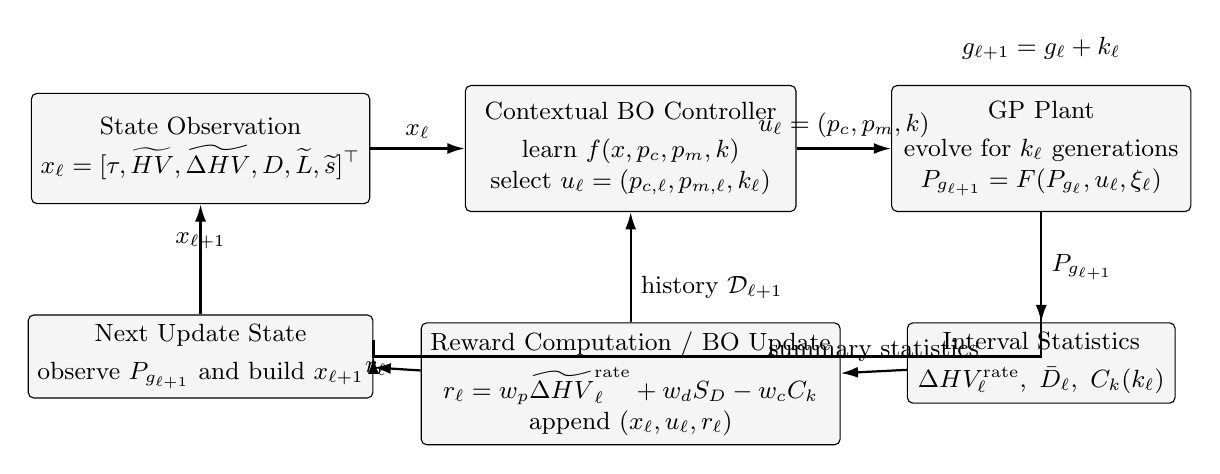
\begin{tikzpicture}[font=\small, node distance=10mm and 12mm]
  \node[block, minimum width=34mm, minimum height=14mm] (obs) {State Observation\\[1mm]
    $x_\ell = [\tau,\widetilde{HV},\widetilde{\Delta HV},D,\widetilde{L},\widetilde{s}]^\top$};
  \node[block, right=of obs, minimum width=42mm, minimum height=16mm] (bo) {Contextual BO Controller\\[1mm]
    learn $f(x,p_c,p_m,k)$\\
    select $u_\ell=(p_{c,\ell},p_{m,\ell},k_\ell)$};
  \node[block, right=of bo, minimum width=38mm, minimum height=16mm] (plant) {GP Plant\\[1mm]
    evolve for $k_\ell$ generations\\
    $P_{g_{\ell+1}} = F(P_{g_\ell},u_\ell,\xi_\ell)$};
  \node[block, below=14mm of plant, minimum width=34mm] (stats) {Interval Statistics\\[1mm]
    $\Delta HV_\ell^{\mathrm{rate}},\ \bar{D}_\ell,\ C_k(k_\ell)$};
  \node[block, below=14mm of bo, minimum width=42mm] (reward) {Reward Computation / BO Update\\[1mm]
    $r_\ell = w_p\widetilde{\Delta HV}^{\mathrm{rate}}_\ell + w_dS_D - w_cC_k$\\
    append $(x_\ell,u_\ell,r_\ell)$};
  \node[block, below=14mm of obs, minimum width=34mm] (nextstate) {Next Update State\\[1mm]
    observe $P_{g_{\ell+1}}$ and build $x_{\ell+1}$};

  \draw[line] (obs) -- node[above] {$x_\ell$} (bo);
  \draw[line] (bo) -- node[above] {$u_\ell=(p_c,p_m,k)$} (plant);
  \draw[line] (plant) -- node[right] {$P_{g_{\ell+1}}$} (stats);
  \draw[line] (stats) -- node[above] {summary statistics} (reward);
  \draw[line] (reward) -- node[left] {$r_\ell$} (nextstate);
  \draw[line] (nextstate) -- node[above] {$x_{\ell+1}$} (obs);
  \draw[line] (plant.south) |- ($(nextstate.east)+(0.0,0.0)$) -- (nextstate.east);
  \draw[line] (reward.north) -- node[right, pos=0.32] {history $\mathcal{D}_{\ell+1}$} (bo.south);

  \node[align=center, above=2mm of plant, font=\small] (time) {$g_{\ell+1}=g_\ell+k_\ell$};
\end{tikzpicture}

\caption{提案手法の閉ループ制御構造。GP をプラント、外側の文脈付きベイズ最適化を制御器とみなし、更新時点の世代状態 $x_\ell$ を観測して、交叉率 $p_c$、突然変異率 $p_m$、次回更新までの世代数 $k$ を同時に決定する。GP はその入力を $k$ 世代の間保持して進化し、区間要約統計から計算された報酬 $r_\ell$ が BO の更新に用いられる。}
\label{fig:closed-loop-architecture}
\end{figure}

図\ref{fig:closed-loop-architecture} に提案手法の全体構造を示す。制御更新時点 $\ell$ において、まず現在の集団 $P_{g_\ell}$ から状態 $x_\ell$ を観測する。次に BO はこの状態を条件として受け取り、次区間で用いる行動 $u_\ell = (p_{c,\ell}, p_{m,\ell}, k_\ell)$ を出力する。ここで $k$ は次回更新までの世代数として一度定義され、その後は更新周期と呼ぶ。GP はその入力を $k_\ell$ 世代の間保持したまま進化し、区間内の挙動を要約する統計量と次更新時点の集団を返す。最後に、それらを用いて報酬 $r_\ell$ を計算し、$(x_\ell, u_\ell, r_\ell)$ を BO に追加する。この循環により、提案法は探索状態に応じて操作強度と更新周期を逐次調整する閉ループ制御として実現される。

\subsection{3.3 状態ベクトルの定義}


外側 BO に渡す状態ベクトルを

\[
x_\ell =
\left[
\tau_\ell,\;
\widetilde{HV}_\ell,\;
\widetilde{\Delta HV}_\ell,\;
D_\ell,\;
\widetilde{L}_\ell,\;
\widetilde{s}_\ell
\right]^\top
\]

と定義する。ここで、$\tau_\ell$ は進化段階、$\widetilde{HV}_\ell$ は現在性能、$\widetilde{\Delta HV}_\ell$ は直近の改善速度、$D_\ell$ は探索多様性、$\widetilde{L}_\ell$ は平均木サイズ、$\widetilde{s}_\ell$ は停滞長を表す。各成分は、現在の GP が探索初期にあるのか、改善が進んでいるのか、停滞しているのか、あるいは複雑化が進んでいるのかを簡潔に要約することを意図している。

各成分は次のように定義する。

\[
\tau_\ell = \frac{g_\ell}{T}
\]

\[
\widetilde{HV}_\ell =
\mathrm{clip}
\left(
\frac{HV_\ell - HV_{\min}}{HV_{\max} - HV_{\min}},
0, 1
\right)
\]

\[
\widetilde{\Delta HV}_\ell =
\mathrm{clip}
\left(
\frac{HV_\ell - HV_{\ell-1}}{\delta_{HV}},
-1, 1
\right)
\]

\[
\widetilde{L}_\ell =
\mathrm{clip}
\left(
\frac{\bar{L}_\ell}{L_{\mathrm{ref}}},
0, 1
\right)
\]

\[
\widetilde{s}_\ell =
\mathrm{clip}
\left(
\frac{s_\ell}{s_{\max}},
0, 1
\right)
\]

ここで $\tau_\ell$ は総世代数に対する現在位置を表し、$\widetilde{HV}_\ell$ は到達している性能水準を表す。$\widetilde{\Delta HV}_\ell$ は直近区間での改善速度を表し、$\widetilde{L}_\ell$ は bloat の進行度合いを、$\widetilde{s}_\ell$ は停滞の長さを表す。これらを正規化して用いることで、BO への入力スケールを大まかに揃え、異なる問題設定間でも比較的扱いやすい文脈表現を得る。

多様性 $D_\ell$ の第一候補としては構造多様性を用いる。これは、交叉と突然変異が直接作用する対象がプログラム木構造であるためであり、制御入力と観測量の因果関係を比較的素直に捉えやすいからである。集団 $P_{g_\ell} = \{T_1,\dots,T_{N_\ell}\}$ に対し、構造多様性を

\[
D_\ell
=
1
-
\frac{2}{N_\ell(N_\ell-1)}
\sum_{1 \le i < j \le N_\ell}
Sim_g(T_i,T_j)
\]

と定義する。ここで、2 個体 $T_i$ と $T_j$ の構造類似度 $Sim_g$ は

\[
Sim_g(T_i,T_j)
=
\frac{|M(T_i,T_j)|}{|T_i| + |T_j| - |M(T_i,T_j)|}
\]

で与える。$\lvert M(T_i,T_j)\rvert$ は両個体で共有される同型部分木の数である。このような状態ベクトルにより、提案法では進化段階、性能、改善速度、多様性、複雑度、停滞を最小限の次元で同時に表現する。

\subsection{3.4 行動と制約}


本研究の行動は

\[
u_\ell = (p_{c,\ell}, p_{m,\ell}, k_\ell)
\]

である。すなわち、提案法は交叉率と突然変異率に加え、更新周期 $k$ も制御対象に含める。ここで $k$ は単なる効率化変数ではなく、状態が安定している場面では更新を粗くし、状態変化が大きい場面では更新を密にするための制御入力である。したがって、提案法は「どの操作率を使うか」と「いつ次の更新を行うか」を一体として決定する。

行動の探索空間は

\[
\mathcal{U}(x_\ell)
=
\left\{
(p_c,p_m,k)
\mid
p_c \in [p_c^{\min}, p_c^{\max}],
\;
p_m \in [p_m^{\min}, p_m^{\max}],
\;
k \in \mathcal{K},
\;
p_c + p_m \le 1
\right\}
\]

とする。ここで $p_c$ と $p_m$ は連続変数、$k$ は有限離散集合 $\mathcal{K}$ 上の離散変数として扱う。制約 $p_c + p_m \le 1$ は、再生産や他の操作へ割り当てる確率を残すための自然な制約である。初稿段階では具体的な上下限や $\mathcal{K}$ の候補値は固定しないが、提案法の定義としては、連続な操作強度と離散な更新周期を含む混合空間を BO が扱う点を重視する。

\subsection{3.5 報酬関数}


BO が最大化する目的は、区間内の進捗を主としつつ、多様性維持を副次的に評価し、過剰な更新頻度を弱く抑制する単一スカラー報酬である。ここで $k$ を行動に含める以上、単純な区間総 HV 改善量

\[
HV_{\ell+1} - HV_\ell
\]

をそのまま用いると、大きい $k$ を選ぶほど長い区間で改善量を稼ぎやすくなり、更新周期の比較が不公平になりやすい。そこで、本研究では進捗主項として世代あたり改善量を用いる。

\[
\Delta HV^{\mathrm{rate}}_\ell
=
\frac{HV_{\ell+1} - HV_\ell}{k_\ell}
\]

\[
\widetilde{\Delta HV}^{\mathrm{rate}}_\ell
=
\mathrm{clip}
\left(
\frac{\Delta HV^{\mathrm{rate}}_\ell}{\delta_{HV}^{\mathrm{rate}}},
-1, 1
\right)
\]

この定義により、$k$ の長短による有利不利をある程度抑えつつ、区間ごとの進捗効率を比較できる。

多様性項には区間終点の 1 点ではなく、区間平均多様性を用いる。

\[
\bar{D}_\ell
=
\frac{1}{k_\ell}
\sum_{j=1}^{k_\ell}
D_{\ell,j}
\]

多様性は常に高ければよいわけではなく、探索初期では高め、収束期ではやや抑えめが望ましい可能性がある。そこで、世代進行に応じた目標多様性

\[
D^\ast(\tau)
=
D_{\mathrm{start}}
-
(D_{\mathrm{start}} - D_{\mathrm{end}})\tau
\]

を設定し、その整合度を

\[
S_D(\bar{D}_\ell,\tau_{\ell+1})
=
\exp
\left(
-
\left(
\frac{\bar{D}_\ell - D^\ast(\tau_{\ell+1})}{\sigma_D}
\right)^2
\right)
\]

で評価する。これにより、単純な「多様性最大化」ではなく、進化段階に応じた適度な多様性維持を報酬に反映できる。

制御更新コスト項は

\[
C_k(k_\ell)
=
\frac{k_{\max} - k_\ell}{k_{\max} - k_{\min}}
\]

とする。$k$ が小さいほど BO を頻繁に呼び出す必要があり、更新頻度は高くなるため、コストは大きくなる。もっとも、本研究の主張の中心は性能改善と多様性維持の両立にあるため、この項は主項ではなく弱い抑制項として扱う。

以上より、最終報酬は

\[
r_\ell
=
w_p \widetilde{\Delta HV}^{\mathrm{rate}}_\ell
+
w_d S_D(\bar{D}_\ell,\tau_{\ell+1})
-
w_c C_k(k_\ell)
\]

とする。ここで $w_p > w_d > w_c$ を基本方針とし、進捗を主、多様性維持を副、制御コストを抑制項とする。この構成により、提案法は性能偏重にも多様性偏重にも寄り過ぎない形で、状態依存の制御判断を学習できる。

\subsection{3.6 文脈付き BO による制御則}


制御器は標準的なガウス過程ベースの文脈付き BO とする。入力は状態と行動を連結した

\[
z_\ell = [x_\ell, u_\ell]
\]

であり、履歴データを

\[
\mathcal{D}_n = \{(z_i, r_i)\}_{i=1}^{n}
\]

とする。BO は

\[
r_\ell = f(z_\ell) + \varepsilon_\ell
\]

を学習し、現在状態 $x_\ell$ を固定したうえで

\[
u_\ell^\ast
=
\arg\max_{u \in \mathcal{U}(x_\ell)}
\mathrm{EI}(x_\ell, u \mid \mathcal{D}_\ell)
\]

により次行動を選ぶ。

ここで重要なのは、本研究が最適化している対象が

\[
f(p_c,p_m,k)
\]

ではなく、

\[
f(x_\ell,p_c,p_m,k)
\]

である点である。すなわち、同じ $(p_c,p_m,k)$ であっても、現在の探索状態が探索初期、停滞期、収束期のいずれにあるかによって、その行動の有効性は異なるという立場を採る。この点が、非文脈 BO との差分の中心となる。

また、本研究では $k$ を先に決め、その後に $(p_c,p_m)$ を決める階層型ではなく、$(p_c,p_m,k)$ を 1 つの行動として混合空間上で同時に最適化する。この方針により、提案法は「操作強度」と「更新周期」を分離せずに扱うことができ、状態に応じた制御の一貫性を保ちやすい。したがって、提案法の新規性は、BO による単なるパラメータ探索ではなく、状態条件付きで操作率と更新周期を同時に切り替える文脈付き制御にある。

\subsection{3.7 アルゴリズム概要}


\begin{figure}[t]
\centering
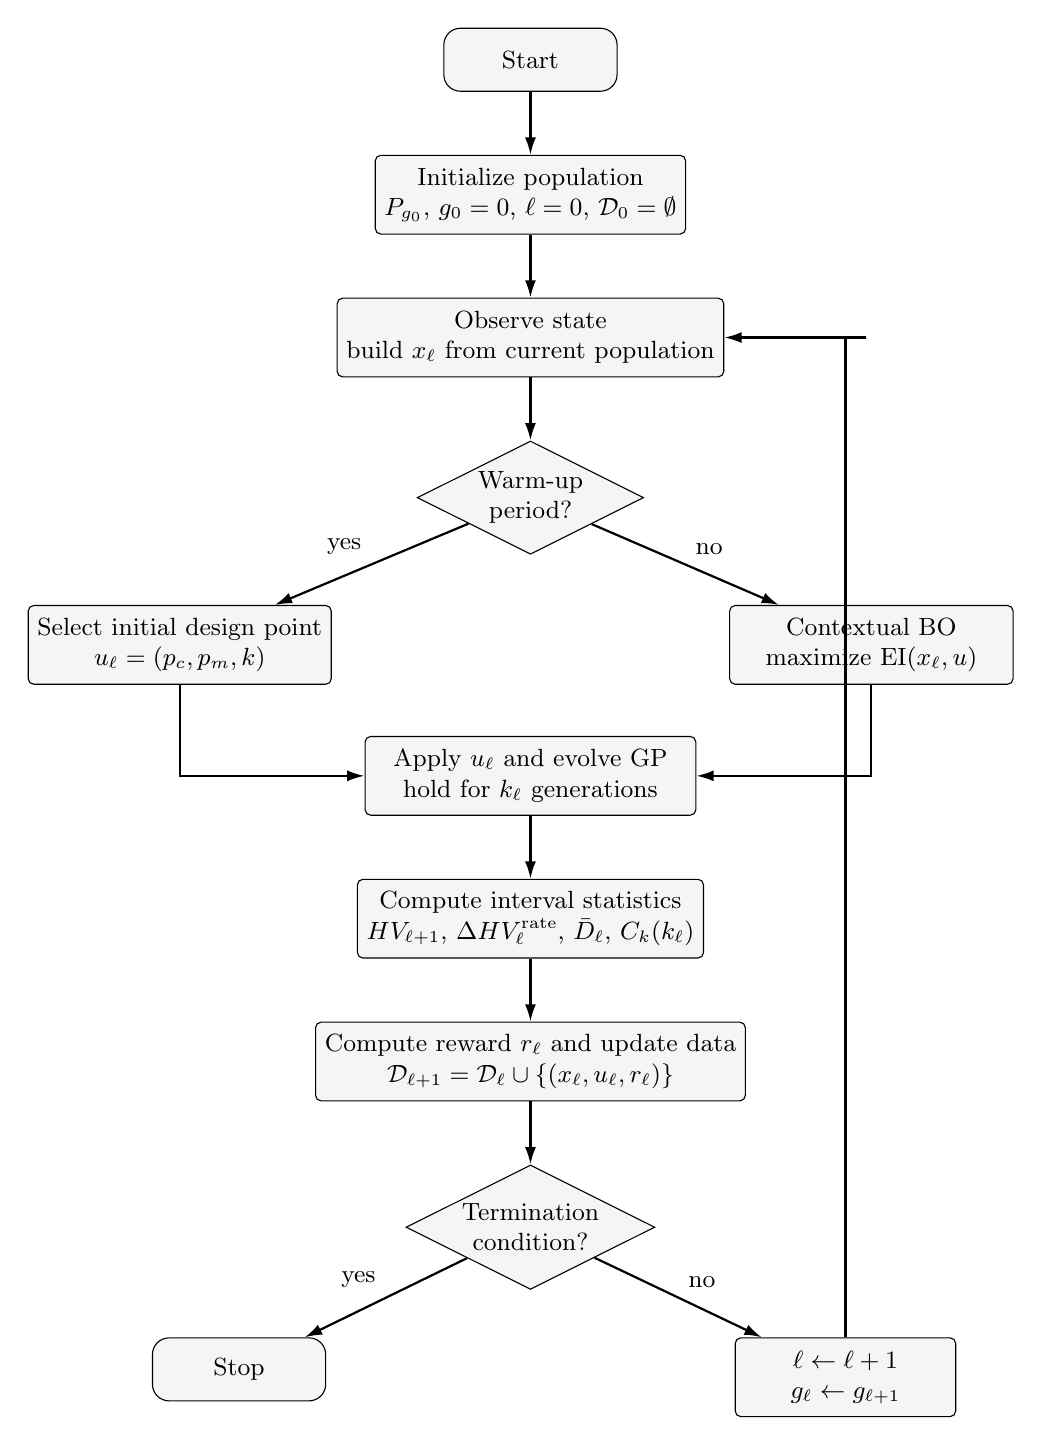
\begin{tikzpicture}[font=\small, node distance=8mm and 20mm]
  \node[terminator] (start) {Start};
  \node[block, below=of start, minimum width=38mm] (init) {Initialize population\\
    $P_{g_0}$, $g_0=0$, $\ell=0$, $\mathcal{D}_0=\emptyset$};
  \node[block, below=of init, minimum width=38mm] (observe) {Observe state\\
    build $x_\ell$ from current population};
  \node[decision, below=of observe, minimum width=24mm] (warmup) {Warm-up\\period?};
  \node[block, below left=10mm and 18mm of warmup, minimum width=34mm] (design) {Select initial design point\\
    $u_\ell=(p_c,p_m,k)$};
  \node[block, below right=10mm and 18mm of warmup, minimum width=36mm] (bo) {Contextual BO\\
    maximize $\mathrm{EI}(x_\ell,u)$};
  \node[block, below=23mm of warmup, minimum width=42mm] (evolve) {Apply $u_\ell$ and evolve GP\\
    hold for $k_\ell$ generations};
  \node[block, below=of evolve, minimum width=42mm] (stats) {Compute interval statistics\\
    $HV_{\ell+1}$, $\Delta HV_\ell^{\mathrm{rate}}$, $\bar D_\ell$, $C_k(k_\ell)$};
  \node[block, below=of stats, minimum width=42mm] (update) {Compute reward $r_\ell$ and update data\\
    $\mathcal{D}_{\ell+1}=\mathcal{D}_\ell \cup \{(x_\ell,u_\ell,r_\ell)\}$};
  \node[decision, below=of update, minimum width=24mm] (stop) {Termination\\condition?};
  \node[terminator, below left=10mm and 18mm of stop] (end) {Stop};
  \node[block, below right=10mm and 18mm of stop, minimum width=28mm] (increment) {$\ell \leftarrow \ell+1$\\
    $g_\ell \leftarrow g_{\ell+1}$};

  \draw[line] (start) -- (init);
  \draw[line] (init) -- (observe);
  \draw[line] (observe) -- (warmup);
  \draw[line] (warmup) -- node[above left] {yes} (design);
  \draw[line] (warmup) -- node[above right] {no} (bo);
  \draw[line] (design) |- (evolve);
  \draw[line] (bo) |- (evolve);
  \draw[line] (evolve) -- (stats);
  \draw[line] (stats) -- (update);
  \draw[line] (update) -- (stop);
  \draw[line] (stop) -- node[above left] {yes} (end);
  \draw[line] (stop) -- node[above right] {no} (increment);
  \draw[line] (increment) |- ([xshift=18mm]observe.east) |- (observe.east);
\end{tikzpicture}

\caption{提案手法の実行フローチャート。初期化後、各更新時点で状態 $x_\ell$ を観測し、warm-up 期間かどうかに応じて初期設計点または文脈付き BO により $(p_c,p_m,k)$ を選択する。続いて GP を $k_\ell$ 世代だけ進化させ、区間統計と報酬を計算し、$(x_\ell,u_\ell,r_\ell)$ を履歴へ追加して終了条件まで反復する。}
\label{fig:proposal-flowchart}
\end{figure}

提案法の処理手順を図\ref{fig:proposal-flowchart} に示す。初期状態では BO の学習データが存在しないため、数点の warm-up 設計点を用いて初期観測を得る。その後は、各更新時点で観測された状態 $x_\ell$ を文脈として、BO が $(p_c,p_m,k)$ を選択する。

図\ref{fig:proposal-flowchart} の流れは次のとおりである。

\begin{enumerate}
\item 初期集団を生成し、$g_0 = 0$、$\ell = 0$ とする。
\item 更新時点の集団 $P_{g_\ell}$ から状態 $x_\ell$ を観測する。
\item warm-up 期間であれば初期設計点から $(p_c,p_m,k)$ を選ぶ。
\item それ以降は、BO が $\mathrm{EI}(x_\ell,u)$ を最大にする $u_\ell = (p_c,p_m,k)$ を選ぶ。
\item $u_\ell$ を固定し、GP を $k_\ell$ 世代だけ進化させる。
\item 次更新時点の集団 $P_{g_{\ell+1}}$ と区間要約統計 $HV_{\ell+1}$, $\Delta HV^{\mathrm{rate}}_\ell$, $\bar{D}_\ell$, $C_k(k_\ell)$ を得る。
\item 報酬 $r_\ell$ を計算し、$(x_\ell,u_\ell,r_\ell)$ を履歴へ追加する。
\item 終了条件を満たすまで $\ell \leftarrow \ell + 1$ として繰り返す。
\end{enumerate}


以上により、提案法は GP の進化状態を観測しながら、操作率と更新周期を逐次調整する状態依存・閉ループ制御として実現される。

\section{4. 比較手法}


\subsection{4.1 比較の考え方}


提案法の有効性を明確に評価するため、本研究では GP の表現、個体数、選択方式、終端条件、評価予算などの基本設定は全手法で共通とし、外側から与える制御方策のみを変化させる。したがって、比較の焦点は GP 本体の差ではなく、交叉率 $p_c$、突然変異率 $p_m$、および更新周期 $k$ をどのような情報に基づいて、どのような規則で決定するかに置かれる。

このように比較軸を揃えることで、提案法が優れていた場合、その要因を「内部表現や選択法の違い」ではなく、「探索状態を観測して操作強度と更新周期を切り替える文脈付き制御の有効性」に帰着しやすくなる。逆に、性能向上が得られなかった場合でも、どの情報を見ても十分な制御改善が得られなかったのか、あるいは BO の学習に必要な観測数が不足したのかを明確に議論しやすい。

\subsection{4.2 固定率 GP}


最も基本的な比較対象は、交叉率と突然変異率を全世代を通じて一定に保つ固定率 GP である。このとき操作入力は

\[
u_g = (\bar{p}_c, \bar{p}_m)
\]

であり、$g$ に依らず不変である。すなわち、固定率法では

\[
u_g = u
\quad
\forall g
\]

が成り立つ。ここでは外側制御器は存在せず、現在の探索状態に応じて操作率を切り替える機構も持たない。

固定率法は実装が簡潔で広く用いられている一方、探索初期と収束期で望ましい操作率が異なる可能性を取り込めない。そのため、本研究では最も基本的かつ不可欠なベースラインとして位置づける。

\subsection{4.3 手設計スケジュール GP}


2 つ目の比較対象は、操作率を事前に定めた世代依存スケジュールに従って変化させる手法である。この場合、操作入力は

\[
u_g = u(g)
\]

と表される。たとえば、探索初期では突然変異率を高め、終盤では交叉率を相対的に重くするような線形スケジュールや、一定世代ごとに操作率を段階的に切り替える区分的スケジュールが考えられる。

この比較対象の重要な点は、時間 $g$ には依存しても、現在の探索状態 $x_\ell$ は参照しないことである。したがって、同じ世代数であれば、集団が停滞している場合も順調に改善している場合も、同じ操作率スケジュールが適用される。更新周期 $k$ についても、固定値あるいは事前に決めた更新時刻列を用いるため、更新の粗密は状態に応じて変化しない。これにより、提案法との差分は「可変かどうか」だけでなく、「状態を見て切り替えるかどうか」として整理できる。

\subsection{4.4 非文脈 BO による制御}


3 つ目の比較対象は、外側に BO を置く点では提案法と同じであるが、現在の探索状態を入力に含めない非文脈 BO である。この手法では、BO が学習する対象は

\[
r = f(p_c,p_m,k)
\]

であり、行動の良し悪しを状態によらず一律に評価する。

非文脈 BO でも、行動空間は提案法と同様に

\[
u_\ell = (p_{c,\ell}, p_{m,\ell}, k_\ell)
\]

とし、$p_c$、$p_m$、$k$ を同時に最適化する。ただし、次行動の選択は過去の $(u_\ell, r_\ell)$ からのみ行われ、更新時点の集団状態 $x_\ell$ は条件として用いない。そのため、この手法は「BO によって操作率探索を自動化する」ことはできるが、「その時点の探索状態に応じて制御方針を切り替える」ことはできない。

この比較対象は本研究において特に重要である。なぜなら、$p_c$、$p_m$、$k$ を BO で最適化するだけでは、提案法の新規性はまだ十分に示せないからである。提案法の核は BO の採用そのものではなく、状態条件付きで行動を評価する文脈付き化にある。したがって、非文脈 BO は主要ベースラインとして位置づけられる。

\subsection{4.5 提案法との差分}


提案法では、BO が学習する対象を

\[
r = f(x_\ell,p_c,p_m,k)
\]

と定義する。ここで $x_\ell$ は更新時点の進行率、現在 HV、直近改善量、多様性、平均木サイズ、停滞長からなる状態ベクトルである。したがって、同じ $(p_c,p_m,k)$ であっても、探索初期、停滞期、収束期といった状態に応じて異なる評価が与えられる。

この点を比較対象と対比すると、各手法の違いは次のように整理できる。

\begin{itemize}
\item 固定率 GP: $u$ は全世代で一定であり、状態依存性を持たない
\item 手設計スケジュール GP: $u = u(g)$ であり世代には依存するが状態は見ない
\item 非文脈 BO: $r = f(p_c,p_m,k)$ を学習し、状態を条件に含めない
\item 提案法: $r = f(x_\ell,p_c,p_m,k)$ を学習し、状態に応じて操作強度と更新周期を同時に切り替える
\end{itemize}


したがって、本研究の比較設計は、「固定か可変か」を比べるだけでなく、「状態を見ない可変制御」と「状態を見て切り替える文脈付き制御」を明確に切り分ける構成になっている。とくに、提案法の優位性が非文脈 BO に対して確認されれば、その効果は BO 導入の一般論ではなく、文脈付き閉ループ制御としての設計に由来すると主張しやすくなる。

\subsection{4.6 仮説との対応}


以上の比較手法は、研究仮説と次のように対応する。

\begin{itemize}
\item 固定率 GP との比較: 状態依存制御そのものの有効性を検証する
\item 手設計スケジュール GP との比較: 世代依存スケジュールではなく状態依存制御であることの意義を検証する
\item 非文脈 BO との比較: BO の導入自体ではなく、文脈付き化の効果を検証する
\end{itemize}


主仮説 $H1$ は、提案法が固定率法および非文脈 BO よりも HV 改善と多様性維持を両立できるかどうかによって評価される。副仮説 $H2$ は、$k$ を制御対象に含めることで、毎世代更新より少ない制御回数でも同等以上の進化性能を達成できるかどうかで評価される。さらに補助仮説 $H3$ は、多様性項を報酬から除いた場合、短期的な HV 改善に偏って早期収束しやすくなるかどうかによって検証される。

以上の比較により、本研究では文脈付き化の効果と更新周期制御の効果を切り分けて検証する。次章では、これらの比較を公平に実施するための問題設定、評価指標、実験条件、および統計的比較方法を定義する。


\end{document}
